\chapter{Concurrency Model}

\label{ch:concurrencymodel}

\section{Workers}
    All workers inherit the Peasant class which is nothing more than a specialized Thread.

    Here are the workers with their more than explicit names:
    \begin{itemize}
        \item FetchWorker - will update your local repository with any changes that appeared on the remote on. Every 5 seconds, will block the SyncWorker, in order to perform the fetch operations. If it successfully retrieved data form the remote repository, will announce the SyncWorker that it has some changes that needed to be merge.
        \item SyncWorker - it responsible with commit creation, merging local changes with the remote ones and push those changes to other repository. If any of this operations fail, the filesystem will be locked into a read-only state.
    \end{itemize}
    
    \begin{figure}[h]
      \begin{center}
        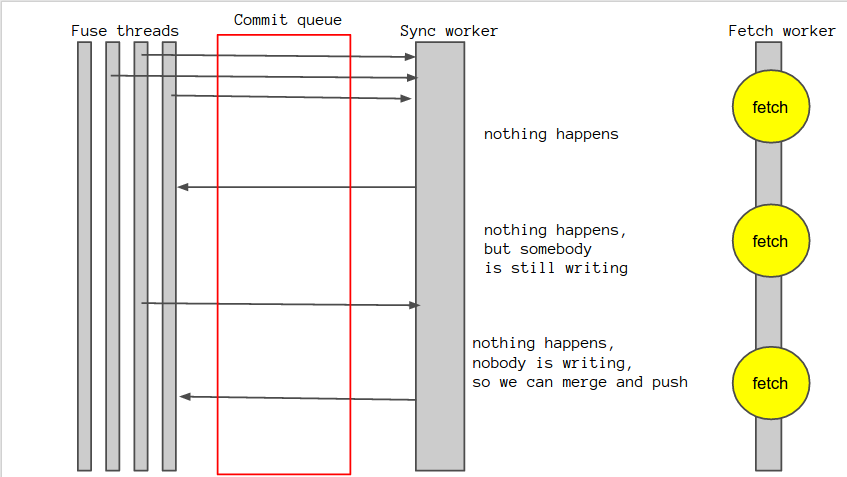
\includegraphics[width=16cm]{concurrency/gitfs.png}
      \end{center}
   \end{figure}
\section{Merging}
\section{Options}
In order to use options when mounting gitfs, you need to append the options as an argument when using the mount command like this: -o option1=value1,option2=value2,option3=value3...

\begin{itemize}
    \item remote\_url: the URL of the remote
    \item branch: the branch name to follow (default: master)
    \item repo\_path: the location where the repositories will be cloned
    (default: $/var/lib/gitfs/repo_path$)
    \item max\_size: the maximum file size in MBs allowed for an individual file. If set to 0, then allow any file size (default: 10MB)
    \item user: the user that will mount the file system (default: root)
    \item group: the group that will mount the file system (default: root)
    \item committer\_name: the name that will be displayed for all the commits (default: user)
    \item committer\_email: the email that will be displayed for all the commits (default: user@FQDN)
    \item merge\_timeout:	the interval between idle state and commits/pushes (default: 5s)
    \item fetch\_timeout: 	the interval between fetches (default: 30s)
    \item log: the path of the log file. Special name syslog will log to the system logger (default: syslog)
    \item log\_level: the logging level. One of error, warning, info, debug (default: warning)
    \item debug: he switch that sets the log level to debug and also enables FUSE’s debug (default: false)
    \item username: the username for HTTP basic auth 
    \item password: the password for HTTP basic auth
    \item key:the path of the SSH private key. NOTE: the public key is constructed by appending .pub to this path and the file MUST exist (default: \textdollar HOME/.ssh/id\_rsa)
\end{itemize}